\chapter{Angle Chasing}
Geometry and I have a relation which the less spoken about, the better. We don't get along. While I have a better appreciation for geometry now, I still am somewhat fearful of it. The main reason of my problems with Geometry is fundamentally due to the fact that I memorized theorems early on without understanding(or reading the proof) in many cases.\\
This is something you need to avoid from the get go. \\
This chapter is about one of the most critical skills for a geometer. Using data about some angle to find others by chasing. We'll learn geometry through problems rather than through theorems,\\
A lot of angle chasing is easier to actually solve then to follow from the solution, so maybe ignore my answers and try to solve everything yourself...\\
\section{Triangle Centers}
We can define the center of triangle in a lot of ways, this leads to there being many centers of the same triangle each one correct based on some criterion.\\
We'll talk about $4$ such centers now.\\
\begin{figure}
    \centering
    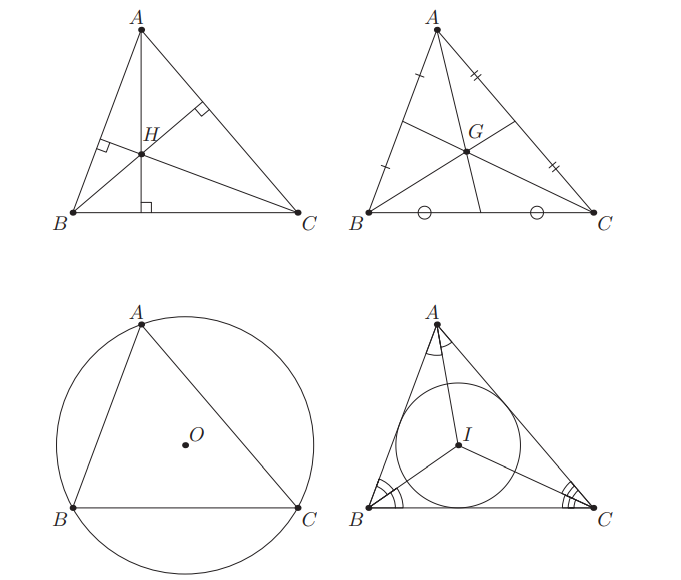
\includegraphics[width=0.75\linewidth]{Photos/Triangle Centers.png}
    \caption{The four primitive centers}
    
\end{figure}
\begin{definition}
    \begin{itemize}
        \item The orthocenter of $ABC$, usually denoted by $H$, is the intersection of the perpendiculars (or altitudes) from $A$ to $BC$, $B$ to $CA,$ and $C$ to $AB$. The triangle formed by the feet of these altitudes is called the orthic triangle. 
        \item The centroid, usually denoted by $G$, is the intersection the medians, which are the lines joining each vertex to the midpoint of the opposite side. The triangle formed by the midpoints is called the medial triangle.
        \item The incenter, usually denoted by $I$ , is the intersection of the angle bisectors of the angles of $ABC$. It is also the center of a circle (the incircle) tangent to all three sides. The radius of the incircle is called the inradius.
        \item The circumcenter, usually denoted by $O$, is the center of the unique circle (the circumcircle) passing through the vertices of $ABC$. The radius of this circumcircle is called the circumradius. 
    \end{itemize}
\end{definition}

\section{Cyclic Quadrilaterals}
